\documentclass[12pt,a4paper]{article}
\pagestyle{plain}
\usepackage{fullpage}
\usepackage[english]{babel}
\usepackage{enumerate}

%equations
\usepackage[fleqn]{amsmath}
\numberwithin{equation}{section}

%figures
\usepackage[dvips]{graphicx}
\graphicspath{{./images/}}
\numberwithin{figure}{section}

%excercises
\newcounter{Exercise}
\setcounter{Exercise}{1}
\usepackage[dvipsnames]{xcolor}
\usepackage{framed}
\definecolor{shadecolor}{gray}{0.9}
\usepackage{caption}

%tables
\numberwithin{table}{section}

%specials
\usepackage{textcomp} %special (greek) characters as text
%\usepackage{pstricks} %
%\usepackage{ifthen} %
%\usepackage{calc} %


%document details
\author{N.G. Schultheiss \\ translated and adapted by K. Schadenberg}
\date{}
\title{The Sky}


\begin{document}
\maketitle

\section{Introduction}
This module `The Sky' is a first in a series which includes the `The Universe' and `The Expanding Universe'. This module tries to explain the different ways in which locations of celestial bodies can be defined using angles.

\section{Angles}
\begin{figure}\begin{center}
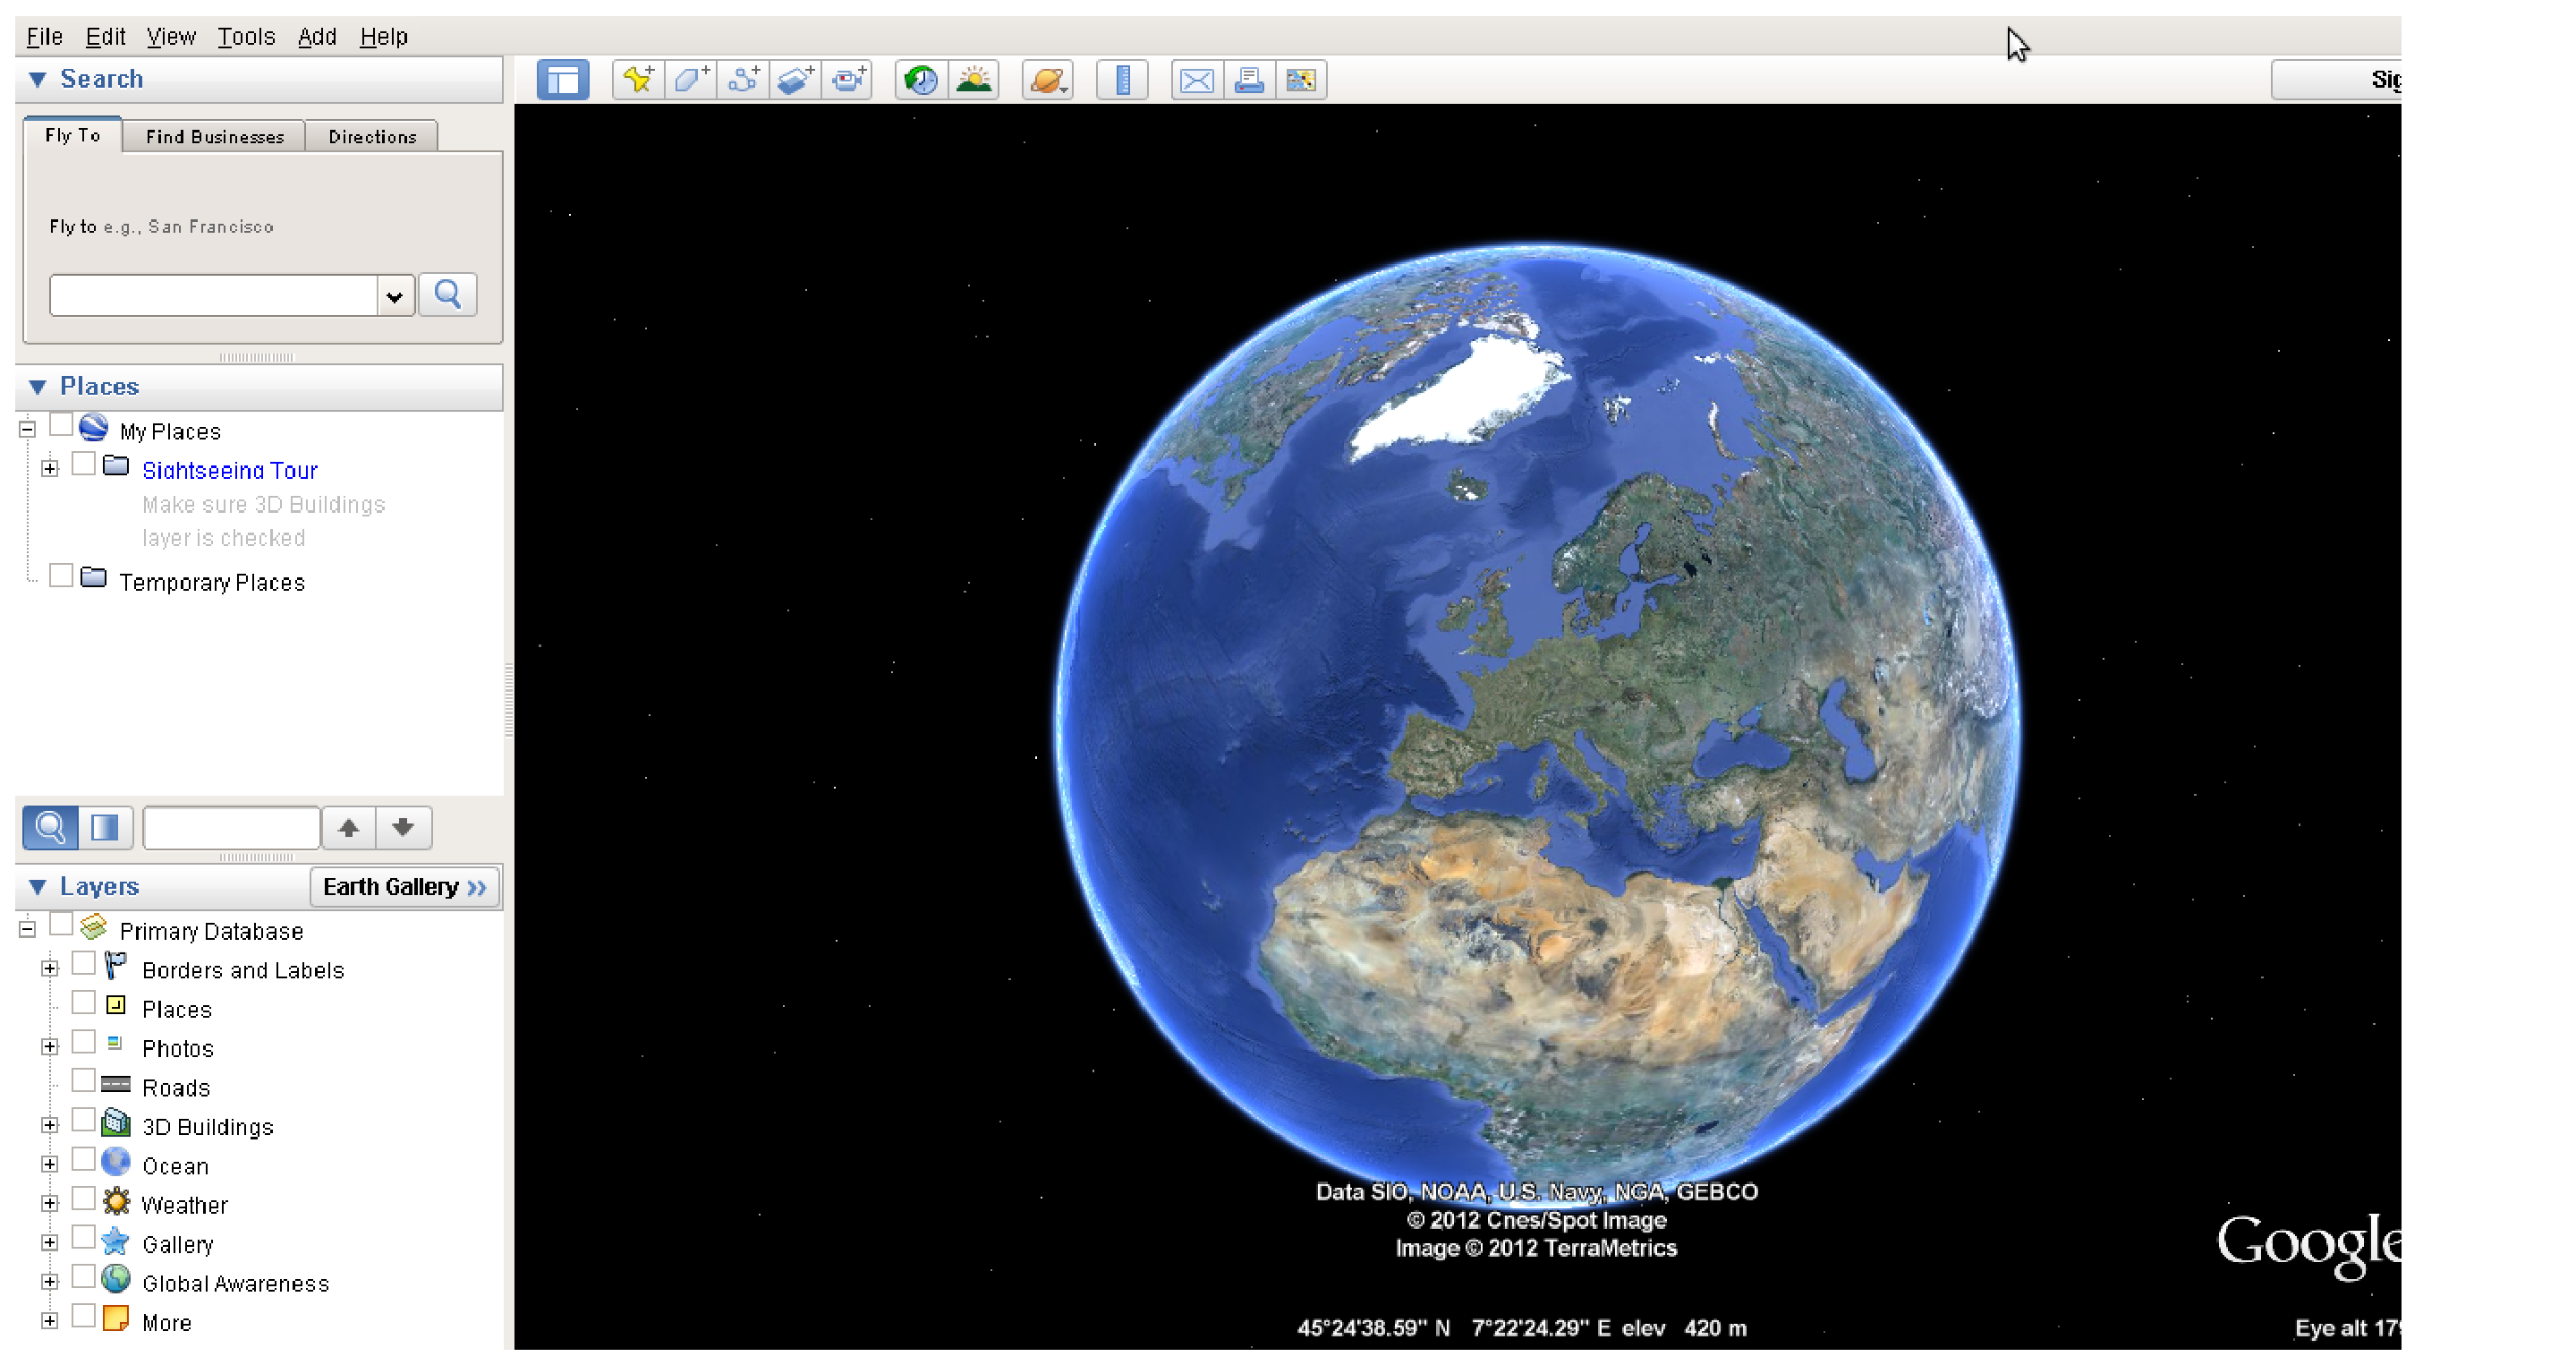
\includegraphics[scale=0.33]{GE_earth.eps}
\caption{The Earth in Google-Earth.}\label{fig:GE_earth}
\end{center}\end{figure} 

In figure \ref{fig:GE_earth} you can see an image of the Earth from the software program Google-Earth. The location 51$^{\circ}$27'29.94'' N 2$^{\circ}$36'07.09'' W points toward the centre of Bristol, the top of the Physics building of the University of Bristol to be exact.\footnote{Also the location of HiSPARC detector 13001.} In this notation the number of degrees North (52) can be easily recognised. The second number in the first set (27) is the number of (arc)minutes. Like an hour, a degree can be divided into 60 (arc)minutes. You can now probably guess what the third number is, the number of (arc)seconds. Using this notation an angle can be represented very accurately.\footnote{An alternative to the number of seconds is decimals of a minute (e.g. 52$^{\circ}$22'.29).}

These angles need to be reported from a specific reference point to indicate a location. We can draw imaginary circles across the surface of the Earth. Lines running from the North to the South pole are called meridians. By definition the prime meridian (or 0$^{\circ}$ meridian) runs through Greenwich in England. The prime meridian divides the Earth into two halves, everything west of this line is on the Western Hemisphere (0$^{\circ}$ to 180$^{\circ}$ West longitude) and every thing to the east is on the Eastern Hemisphere(0$^{\circ}$ to 180 $^{\circ}$ East longitude). All meridians meet at the poles where they intersect at a certain angle. The angle between the meridians running through Greenwich and Bristol is 2$^{\circ}$36'07.09'' towards the West.

With the second number we represent the distance from the equator. We can draw circles across the surface of the Earth which are perpendicular to the meridians; these are circles of latitude. Starting at the equator we need to go 51$^{\circ}$27'29.94'' North to end up in Bristol.

We can convert our notation using degrees, minutes, and second to one which uses only degrees:
\begin{equation*}
4^{\circ}53'35.84'' = 4^{\circ} + \left( \frac{53}{60} \right)^{\circ} + \left( \frac{35.84}{3600} \right)^{\circ} = (4 + 0.883333 + 0.009956)^{\circ} = 4.893289^{\circ}
\end{equation*}

In a similar fashion we can convert an angle using only degrees into one using degrees, minutes, and seconds:
\begin{align*}
& 13.236782^{\circ} = 13^{\circ} + 0.236782^{\circ} \\
& \indent \indent 13^{\circ} + 0.236782^{\circ} = 13^{\circ} + 60 \cdot 0.236782' = 13^{\circ}14' + 0.206921' \\
& \indent \indent \indent \indent 13^{\circ}14' + 0.20692' = 13^{\circ}14' + 60 \cdot 0.20692' = 13^{\circ}14'12.42''
\end{align*}

\begin{shaded}
\textbf{Exercise \theExercise \stepcounter{Exercise}} : We measured an angle of 24.7381$^{\circ}$. Convert this angle into degrees, minutes, and seconds.\end{shaded}
\begin{shaded}
\textbf{Exercise \theExercise \stepcounter{Exercise}} : We measured an angle of 52$^{\circ}$23'17''. Convert this angle into degrees.\end{shaded}

\section{The Sky}
At the top of the Google-Earth window there is a small icon of Saturn. Clicking on this icon shows the stars present in the (night) sky.
\begin{figure}\begin{center}
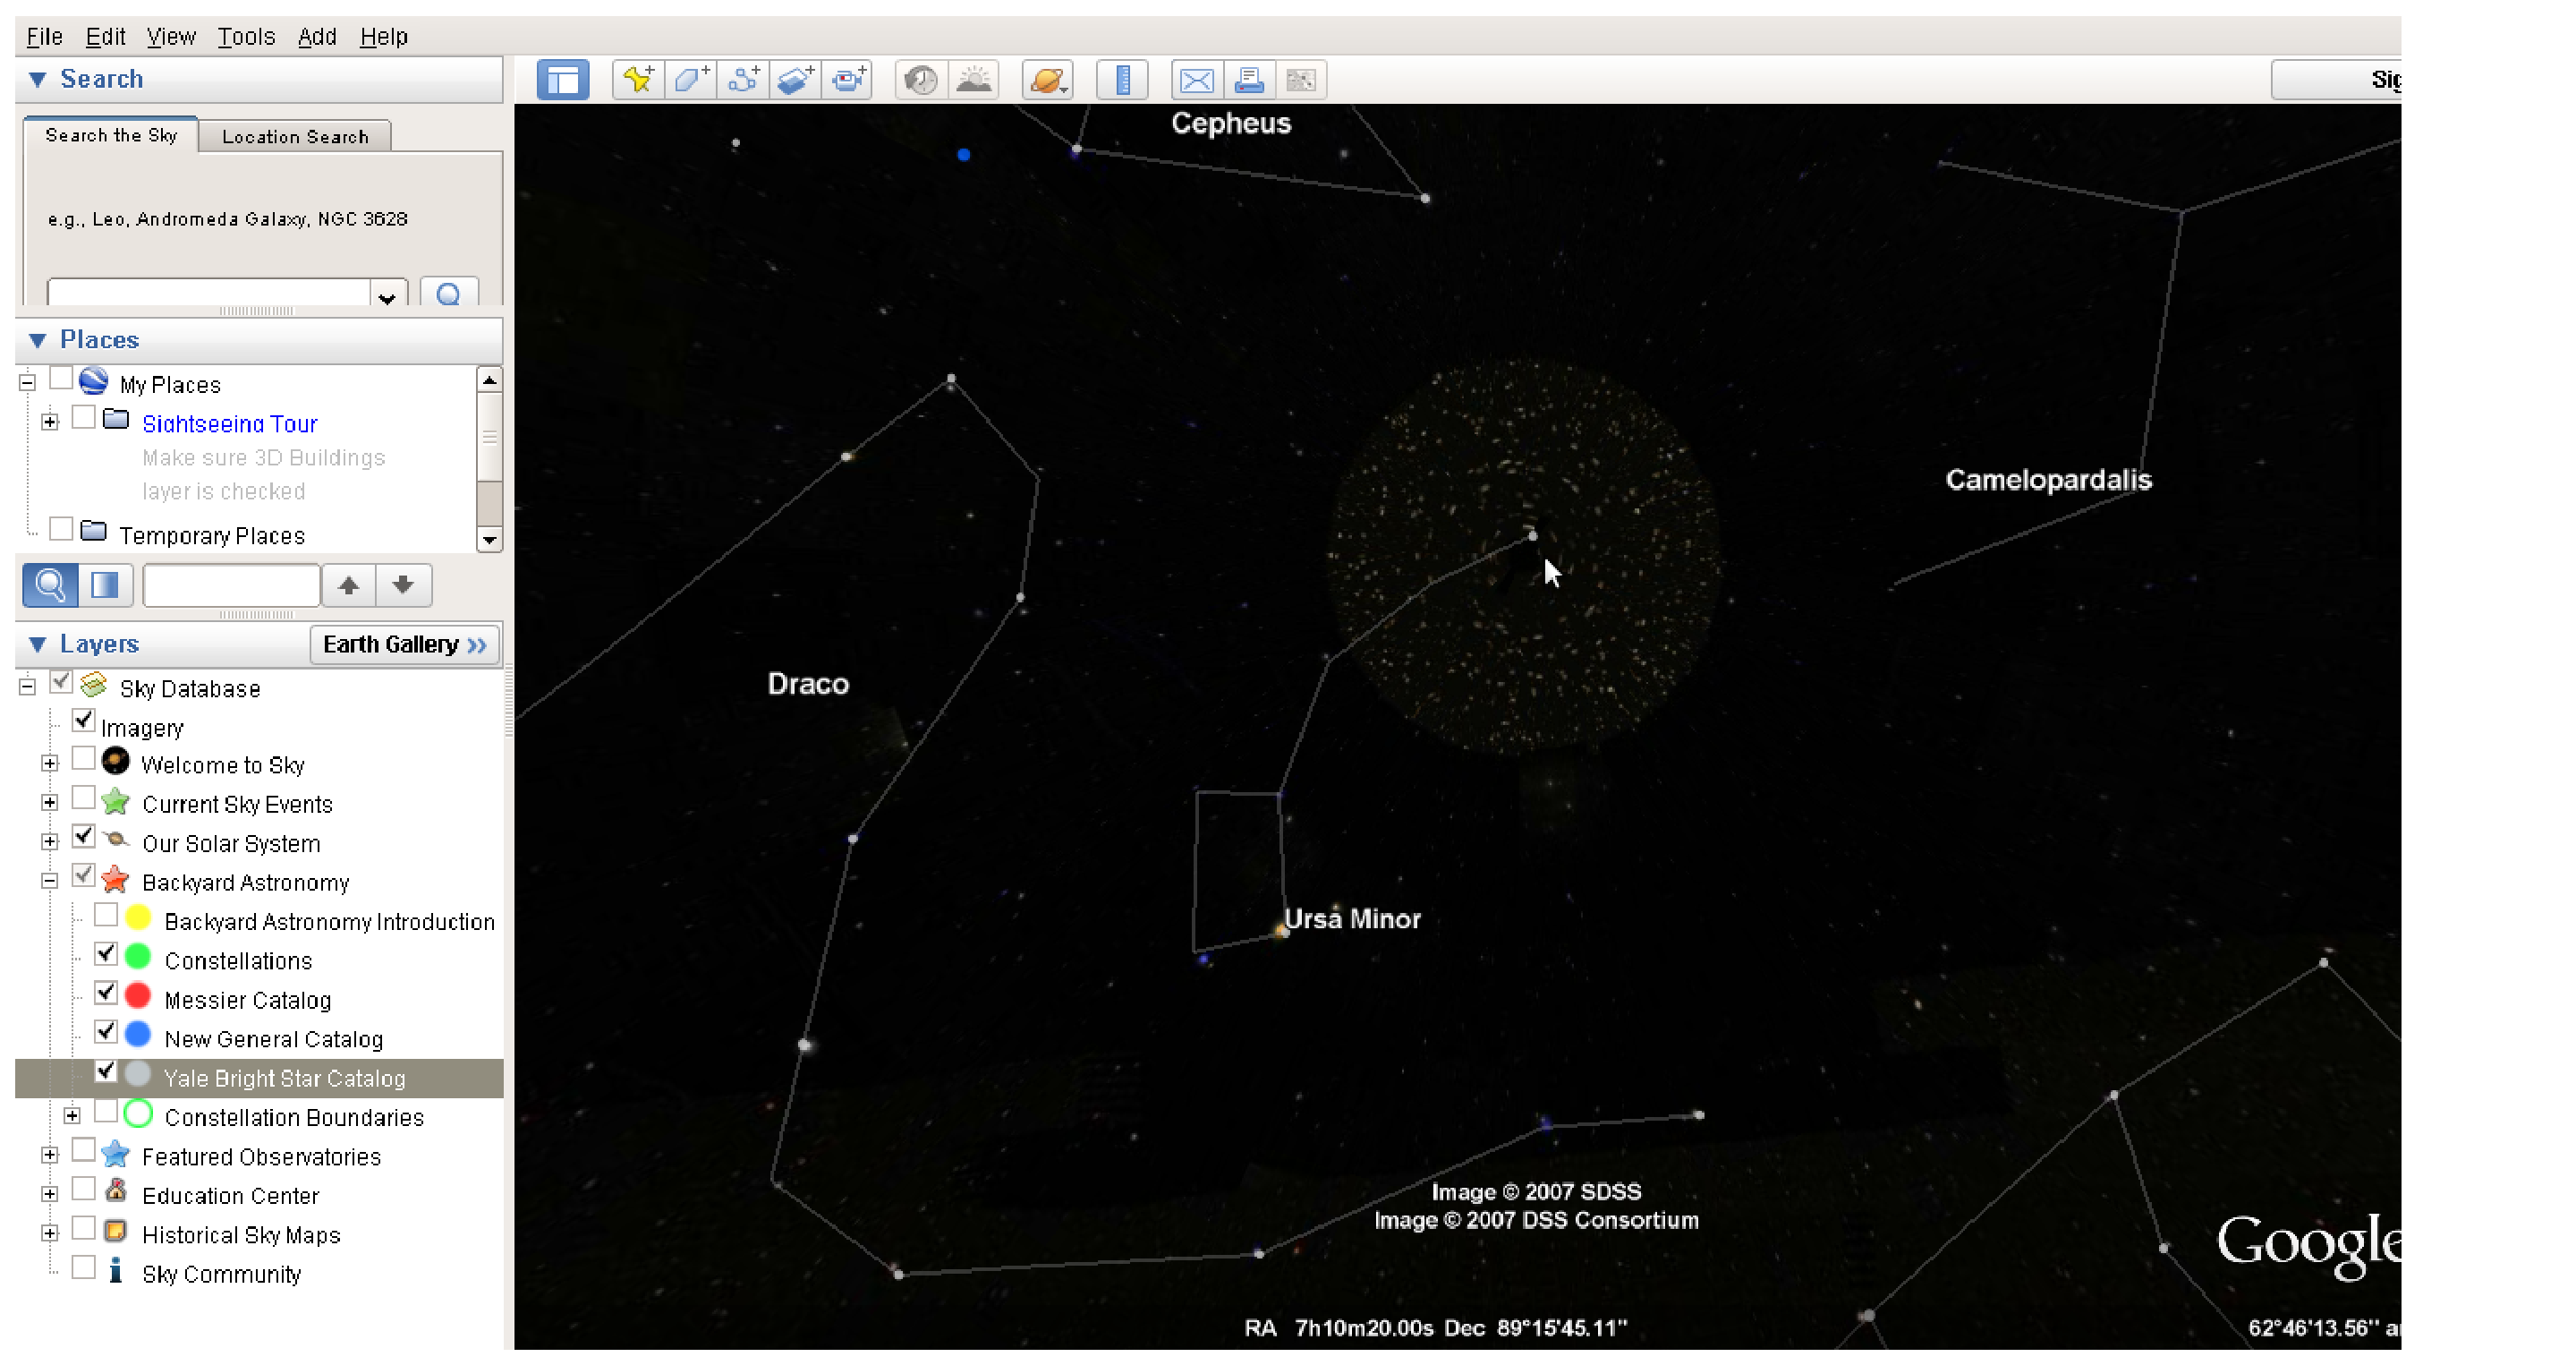
\includegraphics[scale=0.33]{GE_sky.eps}
\caption{The sky according to Google-Earth.}\label{fig:GE_sky}
\end{center}\end{figure}

Figure \ref{fig:GE_sky} shows the stars in the Northern hemisphere. The mouse cursor points towards Polaris, the Pole or North Star. In the bottom of the screen the location of the cursor is represented as RA 7h10m00.00s en Dec 89$^{\circ}$15'45.11''. 

The abbreviation RA stands for Right Ascension, it is the celestial equivalent of the longitude on Earth. Dec is the abbreviation for Declination, this is the celestial equivalent of latitude.

Where are the celestial equator and prime meridian? The celestial equator is the projection of the Earth  equator onto the (imaginary) celestial sphere. Celestial objects on the equator have zero declination. Towards the North pole is positive declination, towards the South pole negative.

The Earth axis of rotation is at an angle with respect to the Sun. This means that the Sun does not move across the Celestial equator but on a different line, called the Ecliptica. The Ecliptoca intersects the Celestial equator two times, at the Spring equinox and Autumnal equinox (also March and September equinox). The Celestial meridians are measured from the Spring equinox.

\begin{shaded}
\textbf{Exercise \theExercise \stepcounter{Exercise}} : Use Google-Earth to look at Ra 0h0m0s Dec 0$^{\circ}$0 0. In which constellation / near which constellation lies this point?\end{shaded}
\begin{shaded}
\textbf{Exercise \theExercise \stepcounter{Exercise}} : Use Google-Earth to look at Ra 2h0m0s Dec 0$^{\circ}$0 0. In which constellation / near which constellation of the zodiac lies this point? Repeat this for 4h0m0s, 6h0m0s, 8h0m0s, 10h0m0s, 12h0m0s, 14h0m0s, 16h0m0s, 18h0m0s, 20h0m0s, and 22h0m0s. List all the names in a table. Observe that the declination of the zodiac is not always 0$^{\circ}$0 0. After 24 hours the circle is complete.\end{shaded}

At the start of Spring the Sun lies in the constellation Pisces.\footnote{According to astrology the Spring equinox lies in the constellation Aries, however the axis of rotation of the Earth has changed in the past 2000 years changing the relative locations.} Celestial time is measured from this point. This time is different from Earth time, which is measured with respect to the Sun. Time measured with respect to the stars is called Sidereal time.

\begin{shaded}
\textbf{Exercise \theExercise \stepcounter{Exercise}} : Complete the following table:
\begin{tabular}{|c|c|}
\hline
\textbf{Earth} & \textbf{Sky} \\
\hline
Length &   \\
\hline
 & Declination \\
\hline
Equator & \\
\hline
\end{tabular}\end{shaded}

\section{Herschel and Messier}
Fredrich Wilhelm Herschel made his living as a musician and wrote multiple symphonies. But he also had a great interest in the sky and therefore build a number of refractor telescopes to study it more closely.

At roughly the same time Charles Messier was also taking a closer look at the skies. He made the now famous list of 110 Messier objects.\footnote{The original list of Messier only contained 103 objects, other astronomers added a further 7.} Messier was a comet hunter, he became frustrated by objects strongly resembling comets but which were in fact not comets. In modern catalogues the original Messier objects can still be recognised by their names; M001 to M110. Herschel was impressed by Messiers work and started doing deep sky (far away) surveys to make his own catalogue. Eventually he published three catalogues together containing over 2500 objects.

\begin{shaded}
\textbf{Exercise \theExercise \stepcounter{Exercise}} : Lets see if we can find one of Herschels objects with Google-Earth. Go to `AR 37 / H969-3' located at RA 11h32m30s Dec +74$^{\circ}$32'. At this exact position you will not find anything, there are however two objects from the NGC list nearby. Can you give an explanation why there is nothing at the location reported by Herschel?\end{shaded}

The first telescopes where rather cumbersome compared to their modern counterparts. In figure \ref{fig:tel_oud} you can see Herschels first telescope. This telescope could only be moved up or down, rotating  involved lifting the entire telescope and repositioning it. If the telescope is precisely aligned along a meridian, the rotation of the Earth makes sure that the telescope can look around the entire sky. A complete circle across the stars takes 24 hours.\footnote{We do have to use the correct time. We can define a day, containing 24 hours, as one rotation of the Earth around its axis with respect to the Sun, but also with respect to the stars. The difference between the two is roughly one day per year, or almost 4 minutes per day. Try to find out why. In the module `Periodical data' you can find more information about the two different time systems.} This is why right ascension is given in a time format and not as an angle. 
\begin{figure}\begin{center}
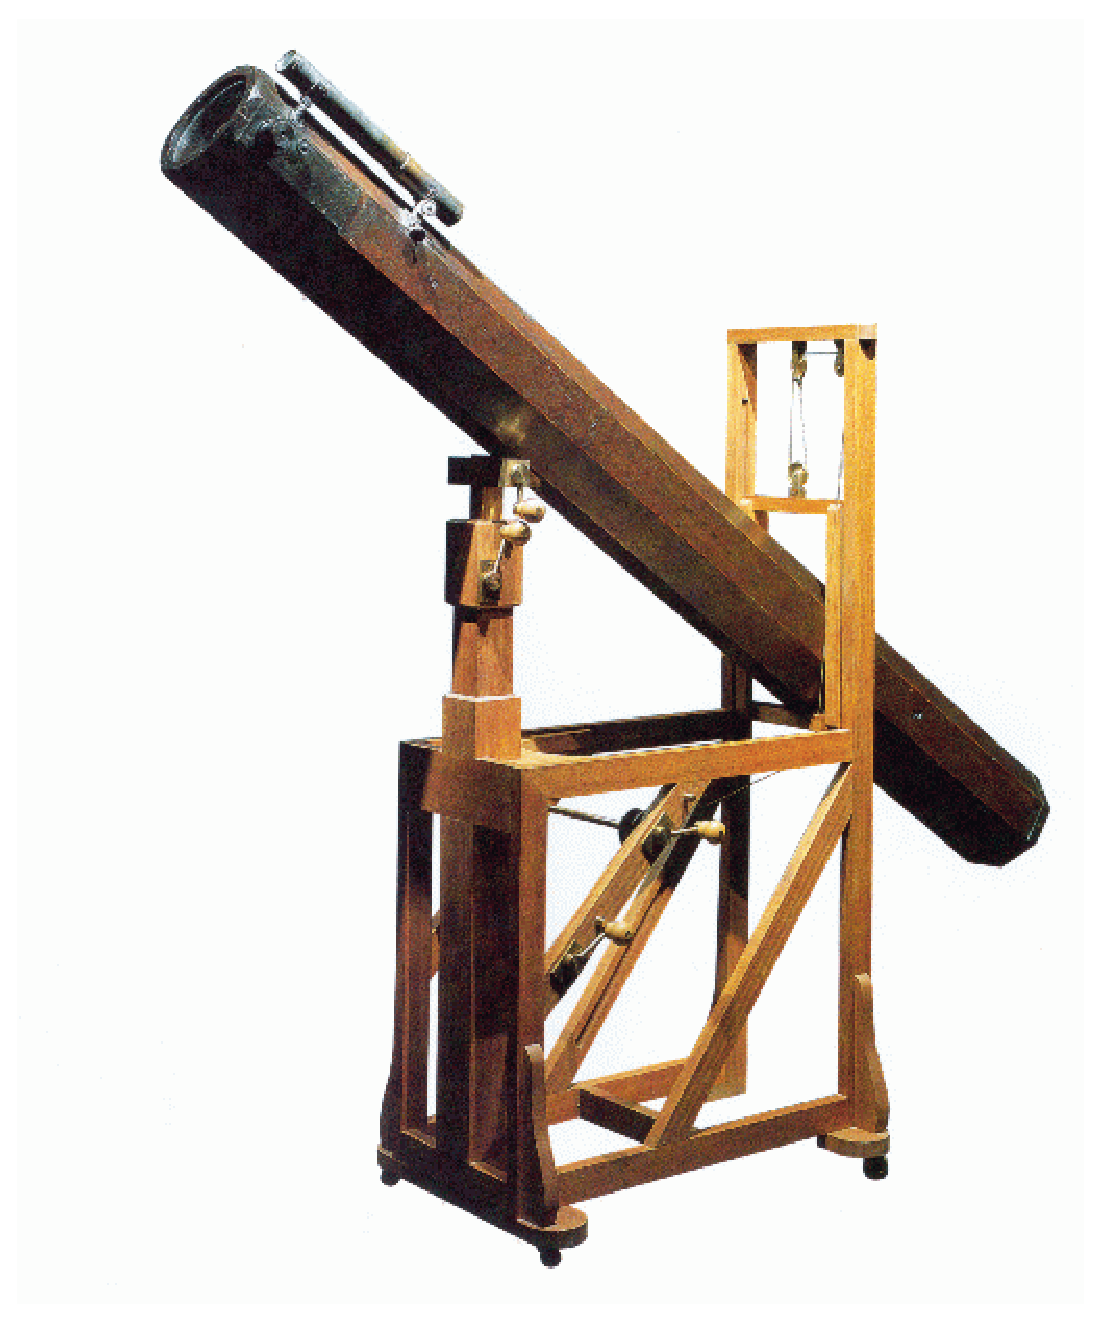
\includegraphics[scale=0.48]{tel_oud.eps}
\caption{Herschels first telescope.}\label{fig:tel_oud}
\end{center}\end{figure} 

\begin{table}[h]
\ttfamily
\tiny
\centering
\begin{tabular}{l l l l l l l l l}
Name & Type & R. A. & Dec & Size & Mag & Con & Herschel \\ \hline
AR 37 & Open cluster & 11:32.5 & +74\~{}32 & & & Dra & H969-3 \\
IC  434 & Nebula & ~5:41.0 & -~2\~{}24 & 60.0 & & Ori & H35-5  Barnard's Loop\\
IC 2995 & Galaxy & 12:05.8 & -27\~{}56 & ~3.1 & 13.5 & Hya & H382-3\\
IC 4051 & Galaxy & 13:00.9 & +28\~{}00 & ~1.1 & 13.2 & Com & H363-3\\
NGC 12 & Galaxy & ~0:08.7 & +~4\~{}37 & ~1.9 & 14.1 & Psc & H868-3\\
NGC 13 & Galaxy & ~0:08.8 & +33\~{}26 & ~2.7 & 13.6 & And & H866-3\\
NGC 14 & Galaxy & ~0:08.8 & +15\~{}49 & ~3.0 & 12.1 & Peg & H591-2\\
NGC 16 & Galaxy & ~0:09.1 & +27\~{}44 & ~2.1 & 12.0 & Peg & H15-4 vF interacting pair\\
NGC 23 & Galaxy & ~0:09.9 & +25\~{}55 & ~2.3 & 12.0 & Peg & H147-3\\
NGC 24 & Galaxy & ~0:09.9 & -24\~{}58 & ~5.5 & 11.5 & Scl & H461-3 Nearly edge-on\\
NGC 29 & Galaxy & ~0:10.8 & +33\~{}21 & ~1.8 & 12.6 & And & H853-2\\
NGC 36 & Galaxy & ~0:11.4 & +~6\~{}23 & ~2.4 & 14.4 & Psc & H456-3\\
NGC 39 & Galaxy & ~0:12.3 & +31\~{}03 & ~1.1 & 13.5 & And & H861-3\\
NGC 40 & Planetary neb & ~0:13.0 & +72\~{}32 & ~~.3 & 10.7 & Cep & H58-4 "400"\\
NGC 52 & Galaxy & ~0:14.6 & +18\~{}33 & ~2.4 & 13.3 & Peg & H183-3  \\
NGC 57 & Galaxy & ~0:15.4 & +17\~{}18 & ~2.6 & 11.6 & Psc & H241-2 = H243-2\\
NGC 61A & Galaxy & ~0:16.5 & -~6\~{}14 & ~1.1 & 14.7 & Psc & H428-3\\
NGC 68 & Galaxy & ~0:18.3 & +30\~{}04 & ~1.5 & 13.0 & And & H16-5\\
NGC 95 & Galaxy & ~0:22.2 & +10\~{}30 & ~1.9 & 12.6 & Psc & H257-2 asym uneven arms\\
\hline
\end{tabular}
\rmfamily
\caption{Part of Herschels catalogue}\label{tab:hers}
\end{table}

\end{document}
